%!TEX program = xelatex
%!TEX root = ./thesis.tex

\section{Experiments on the Flexible-scheduling Hierarchical Method}
This section discusses the experiment results on the proposed flexible-scheduling hierarchical method.

Experiments are done on a set of target tasks: dynamicg8, reachcont and reachcontreg. The target task dynamicg8 is a typical problem that has multi-modality state-space and smooth reward signal, and the target task reachcont is a typical problem that has both multi-modality state-space and sparse reward signal. The set of source tasks is  \{move0, move1, \dots, move7\} for all the experiments.

The problem of hierarchical reinforcement learning consists of two parts: the training of actuator agents and the decider agent. The two problems will be discussed in separate sections.

\subsection{Performance of flat reinforcement learning solutions}
We would firstly like to examine the performance of contemporary reinforcement learning methods on the two typical tasks: dynamicg8 and reachcont. We use the same parameter settings as in section~\ref{sec_exp_adv_reg}. We also test whether exceptional advantage regularization is helpful in these two tasks.

The result on the task dynamicg8 is shown in Figure~\ref{rec_basline_dynamicg8}, and the result on the task reachcont is shown in Figure~\ref{rec_basline_reachcont}. It can be seen that agents fail to solve the tasks. When the task logic becomes more complex and reward function become more sparse, the difficulty of learning useful image features increases, and the task becomes infeasible for contemporary flat reinforcement learning algorithms to solve.

\begin{figure}[!htbp]
	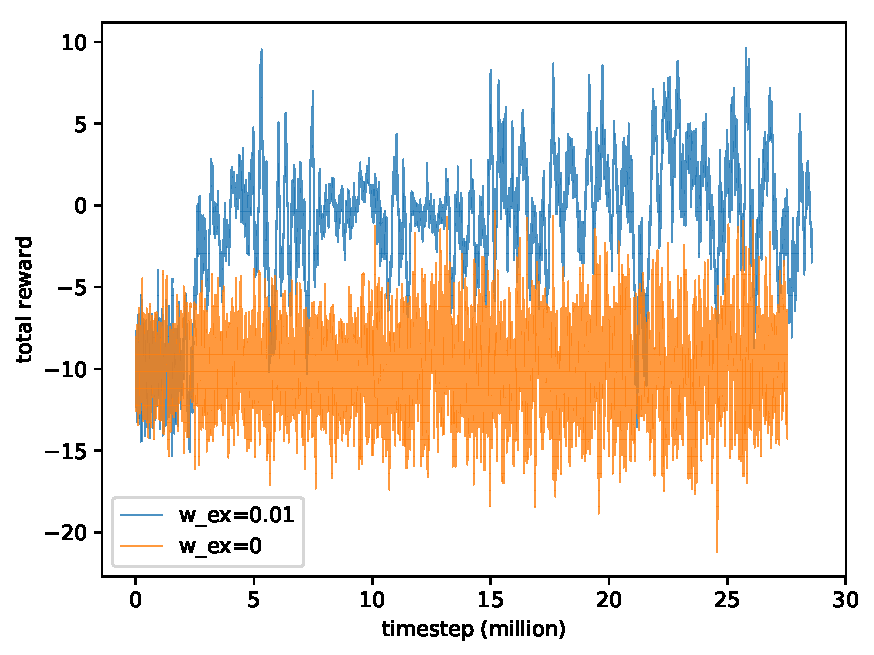
\includegraphics[width=\textwidth]{images/rec_180719_baseline_dynamicg8.pdf}
	\centering
	\caption{Performance of flat reinforcement learning method on the task dynamicg8, with different weights on exceptional advantage regularization. The horizontal axis is the number of million time-steps and the vertical axis is the total episode reward averaged over the last 200 episodes}\label{rec_basline_dynamicg8}
\end{figure}

\begin{figure}[!htbp]
	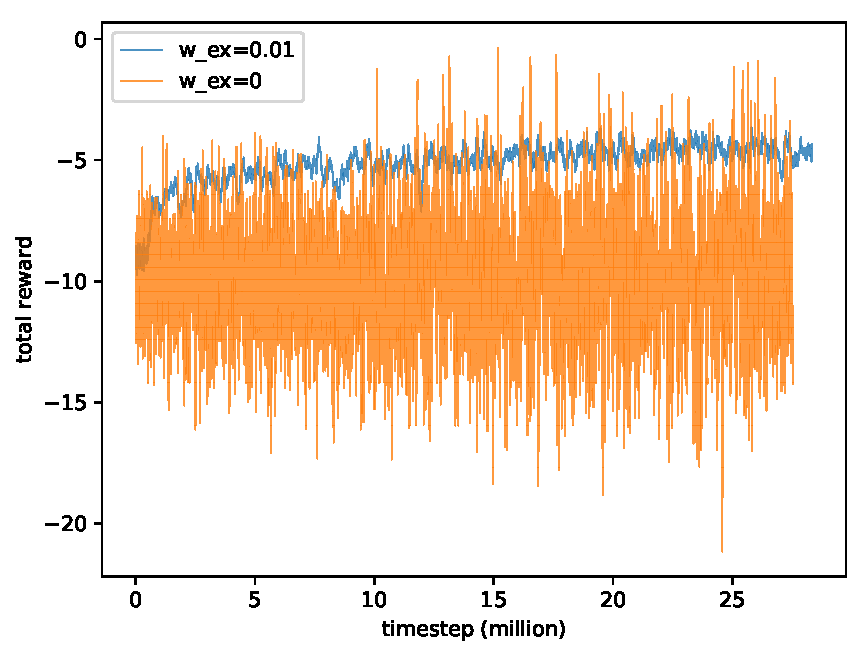
\includegraphics[width=\textwidth]{images/rec_180718_basiline_reachcont.pdf}
	\centering
	\caption{Performance of flat reinforcement learning method on the task reachcont, with different weights on exceptional advantage regularization. The horizontal axis is the number of million time-steps and the vertical axis is the total episode reward averaged over the last 200 episodes}\label{rec_basline_reachcont}
\end{figure}


\subsection{Training the Actuator Agents with Domain Randomization by Cross-sampling Initial States}
As is discussed previously, the learning of the actuator agent of a source task from the source task set is not always the same problem as training a flat reinforcement learning agent for that single task. The initial states generated by actuator agents for other source tasks must be handled, but is usually not encountered in the original source task.

We proposed that the domain randomization by cross-sampling initial states method can handle the problem of novel initial states. The performance of this method is tested in this section. We use the same configuration as in section \ref{sec_exp_move0} for each actuator policy.  

The experiment result on the performance of all the actuator agents is plotted in Figure~\ref{rec_8task_training}. It can be seen that the actuator agents get stuck at sub-optimal performance levels. 

\begin{figure}[!htbp]
	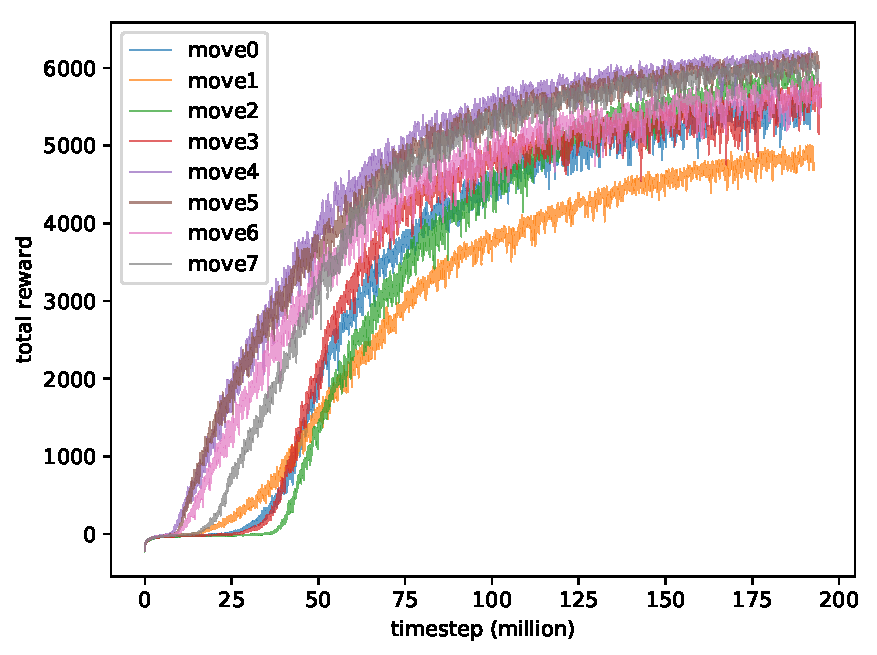
\includegraphics[width=\textwidth]{images/rec_180617_joint8.pdf}
	\centering
	\caption{Performance of actuator agents with domain randomization by cross-sampling initial states, the horizontal axis is the number of million time-steps and the vertical axis is the total episode reward averaged over the last 200 episodes}\label{rec_8task_training}
\end{figure}

Therefore, the proposed synchronous scheduling of actuator learning method aims to prevent this problem. The experiment result of the technique is shown in Figure \ref{rec_sync_training}. In this experiment, the policy training of the actuator agents who outperforms the global lowest-performance by 1000 is paused until all other actuator agents outperform this agent. The result shows that all the actuator agents are able to reach a final performance of around 6000, although the performance of different agents diverge initially. This has verified that the proposed method can successfully prevent any actuator agents getting stuck at sub-optimal performance levels. 

\begin{figure}[!htbp]
	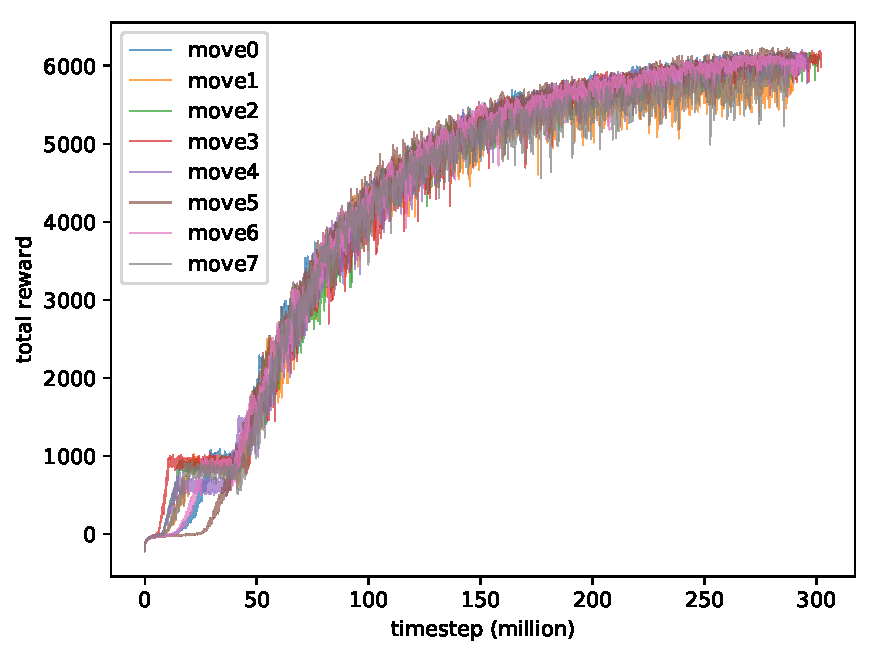
\includegraphics[width=\textwidth]{images/rec_180619_sync.pdf}
	\centering
	\caption{Performance of actuator agents using synchronous scheduling of actuator learning , the horizontal axis is the number of million time-steps and the vertical axis is the total episode reward averaged over the last 200 episodes}\label{rec_sync_training}
\end{figure}

Therefore the learning of source tasks is successfully solved by the proposed technique of domain randomization by cross-sampling initial states with synchronous scheduling of actuator learning method.
\subsection{Training the Decider Agent}
The training of the decider agent consists of two phases: the training of the decision policy and the switcher policy. We train them in two separate phases. In the first phase, the switcher policy is initialized so that it outputs a termination signal whenever the current decision policy has been executed for more than $l_c$ time steps, which is set to 10 in our experiments. The decision policy is trained with the switcher policy being fixed. After the performance of the decision policy converges, the switcher policy is then trained with the decision policy fixed. We train the networks with a PPO algorithm.

\subsubsection{Phase 1: Decision policy training}
The architecture of neural networks is the same as the agent in section \ref{sec_multi_modal_flat} except that the type of distribution is categorical distribution instead of Gaussian distribution.
The experiment result on the performance of the decision policy training on dynamicg8 is shown in Figure~\ref{fig:rec_dynamicg8_decider_subt10}. The result shows that the agent is able to achieve a performance of around 2900. The performance is below the theoretically optimal score of 6000, but the result shows that the agent could at least learn a meaningful policy.

\begin{figure}[!htbp]
\centering
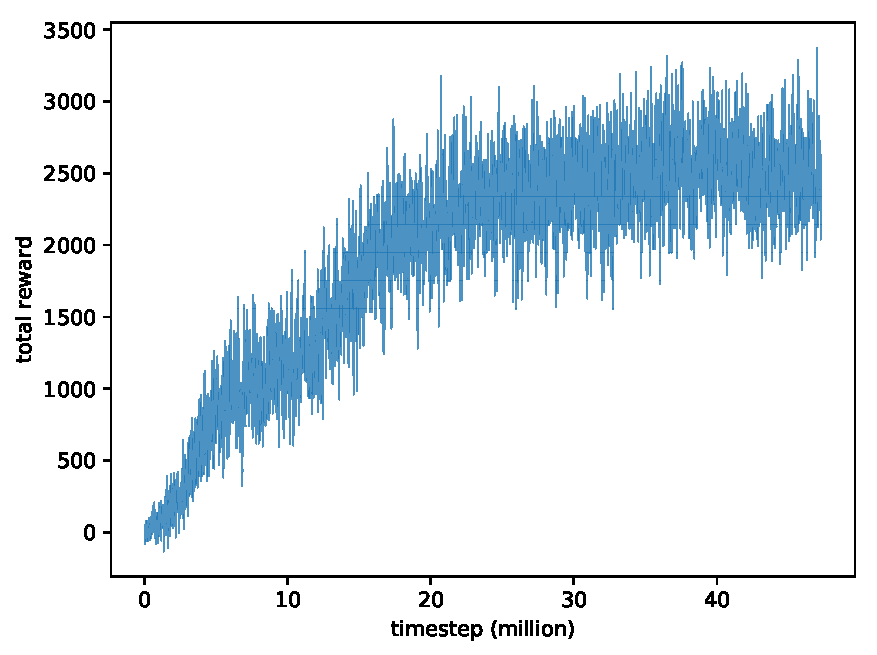
\includegraphics[width=\linewidth]{rec_180630_dynamicg8_exp37}
\caption{Decision policy training performance of the task dynamicg8, the horizontal axis is the number of million time-steps and the vertical axis is the total episode reward averaged over the last 200 episodes}
\label{fig:rec_dynamicg8_decider_subt10}
\end{figure}

The performance of the training of decision policy on task reachcont is shown in Figure~\ref{fig:rec_reachc05_decider_subt10}. The agent achieves an average reward of around 0.75, and is considered having solved the task.
\begin{figure}[!htbp]
\centering
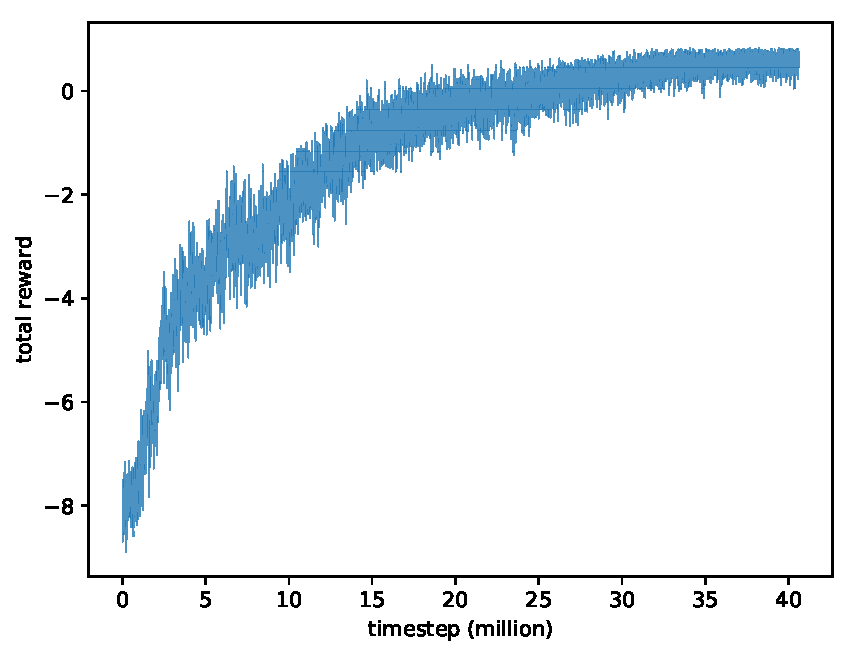
\includegraphics[width=1\linewidth]{rec_0702_reacc05_decider_exp2.pdf}
\caption{Decision policy training performance of the task reachcont, the horizontal axis is the number of million time-steps and the vertical axis is the total episode reward averaged over the last 200 episodes}
\label{fig:rec_reachc05_decider_subt10}
\end{figure}

The performance of the training of decision policy on task reachcontreg is shown in Figure~\ref{rec_reachcontreg}. The task appears to be more difficult than reachcont because the episode length is much longer. The hierarchical reinforcement learning agent still manages to solve the task in the end.
\begin{figure}[!htbp]
	\centering
	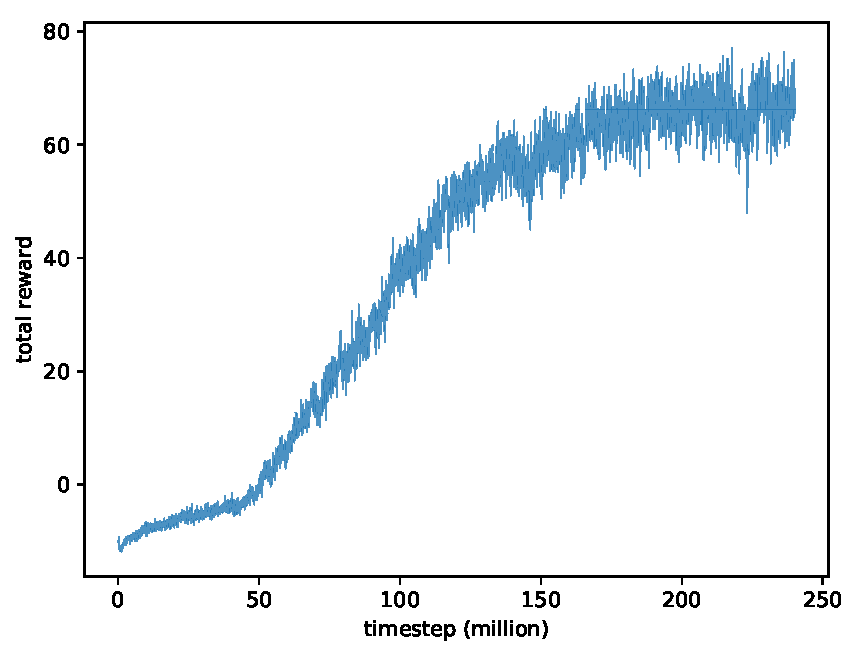
\includegraphics[width=1\linewidth]{rec_180719_reachcont_2.pdf}
	\caption{Decision policy training performance of the task reachcontreg, the horizontal axis is the number of million time-steps and the vertical axis is the total episode reward averaged over the last 200 episodes}
	\label{rec_reachcontreg}
\end{figure}
%\begin{figure}[!htbp]
%	\centering
%	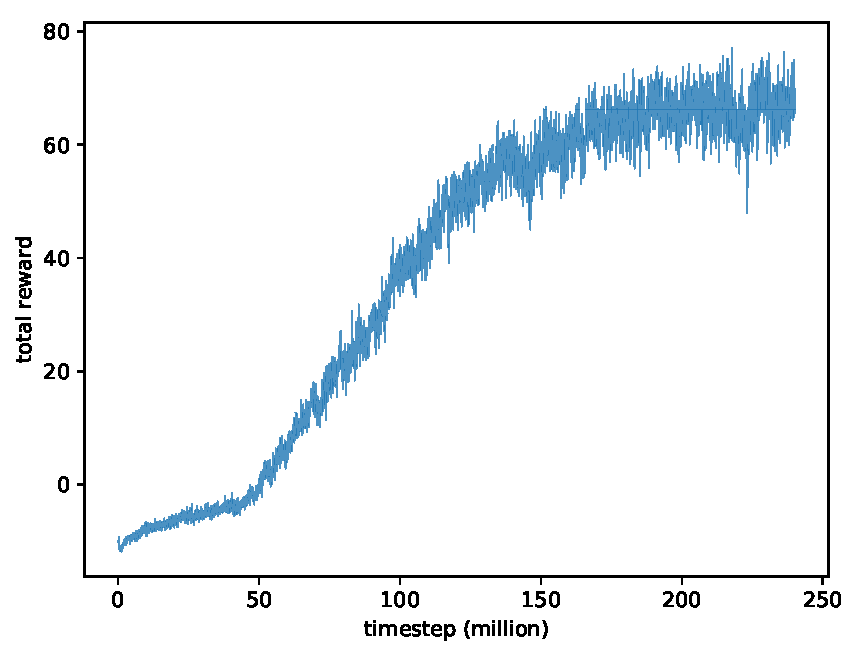
\includegraphics[width=1\linewidth]{rec_180719_reachcont_2.pdf}
%	\caption{Decision policy training performance of the task reachcontreg, the horizontal axis is the number of million time-steps and the vertical axis is the total episode reward averaged over the last 200 episodes}
%	\label{rec_constreachreg}
%\end{figure}

The result of the training of the decision policy shows that the hierarchical reinforcement learning agent is able to achieve a reasonable level of performance. The result is as expected because previous works in SMDP have been studied intensively.

\subsubsection{Phase 2: Switcher policy training}
At the beginning of this phase, the switcher policy is re-initialized randomly so that it outputs a termination signal with a probability of around 0.5. This reinitialized switcher policy is different from the switcher policy in phase 1 which outputs a termination signal deterministically after the current actuator policy has been executed for a pre-defined number of steps. 

The performance of the training of the switcher policy on the task dynamicg8 is shown in Figure~\ref{fig:rec_dynamicg8_switcher}. The best performance during this phase is nearly 3000, which is slightly better than the best performance of 2500 in phase 1. However, the performance suddenly drops to a very low value after around 30 million training steps.

The average execution length of the decision policies is shown in Figure~\ref{fig:rec_dynamicg8_avesubt}. The average execution length becomes around $10$ when the performance reaches the highest level at 30 million training steps, compared to around $4.5$ in phase 1. Therefore, the decision frequency of the decision policy is reduced. It can also be seen that the average execution length suddenly increases to the maximum value 500 after 30 million training steps.

The training of switcher policy is beneficial in the sense that the agent can improve its performance and also reduce the decision frequency of the decision policy. A video recording of the agent with the highest performance can be watched at  the website: [\url{https://youtu.be/ytW7rTpgRAs}].

\begin{figure}[!htbp]
	\centering
	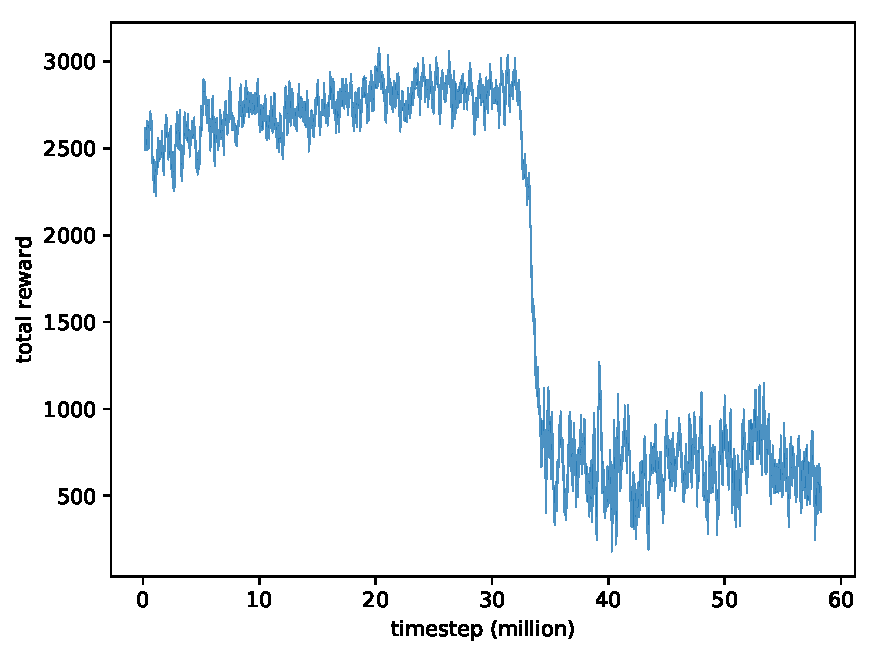
\includegraphics[width=\linewidth]{rec_180707_dynamicg8_switcher_wo_subt}
	\caption{Switcher policy training performance of the task dynamicg8, the horizontal axis is the number of million time-steps and the vertical axis is the total episode reward averaged over the last 200 episodes}
	\label{fig:rec_dynamicg8_switcher}
\end{figure}

\begin{figure}[!htbp]
	\centering
	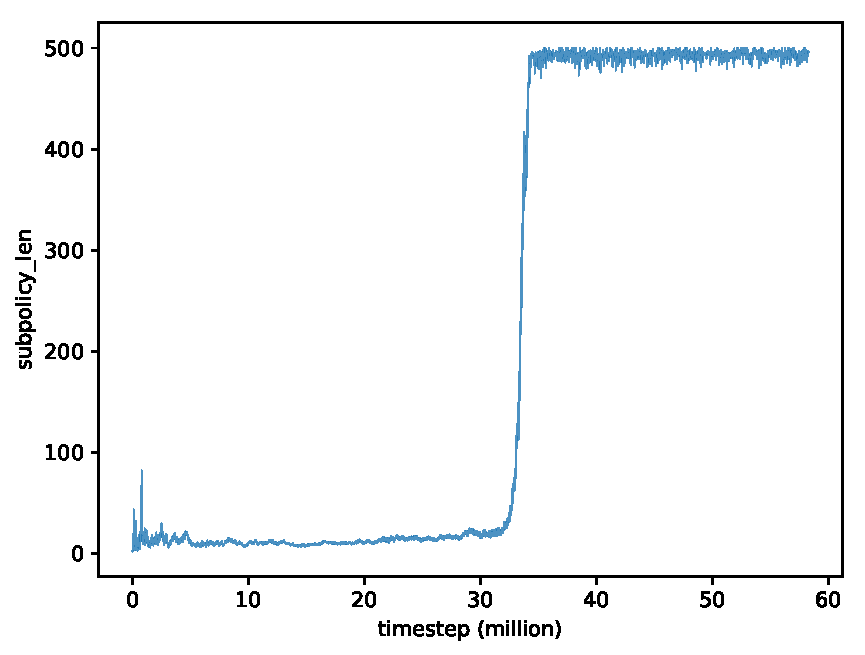
\includegraphics[width=\linewidth]{rec_180707_dynamicg8_switcher_wo_subt_subpolicy_len}
	\caption{Average execution length of the actions of decision policies of the task dynamicg8, the horizontal axis is the number of million time-steps and the vertical axis is the decision policy's average execution length of the last batch.}
	\label{fig:rec_dynamicg8_avesubt}
\end{figure}

The performance of the reachcont switcher policy is shown in Figure~\ref{fig:rec_reachcont_switcher}. The final performance has been improved from $0.75$ in the decision policy training to around $0.81$. The training of switcher policy appears to beneficial to the performance of the target task.

The average execution length of the decision policies is plotted in Figure~\ref{fig:rec_reachcont_switcher_subt}. The final average value of the execution length appears to be reduced to $1.6$, compared to $5$ in the decision policy training phase.

Therefore, the switcher policy is able to improve the reinforcement learning performance at the expense of increasing the decision frequency of the decision policy.

\begin{figure}[!htbp]
	\centering
	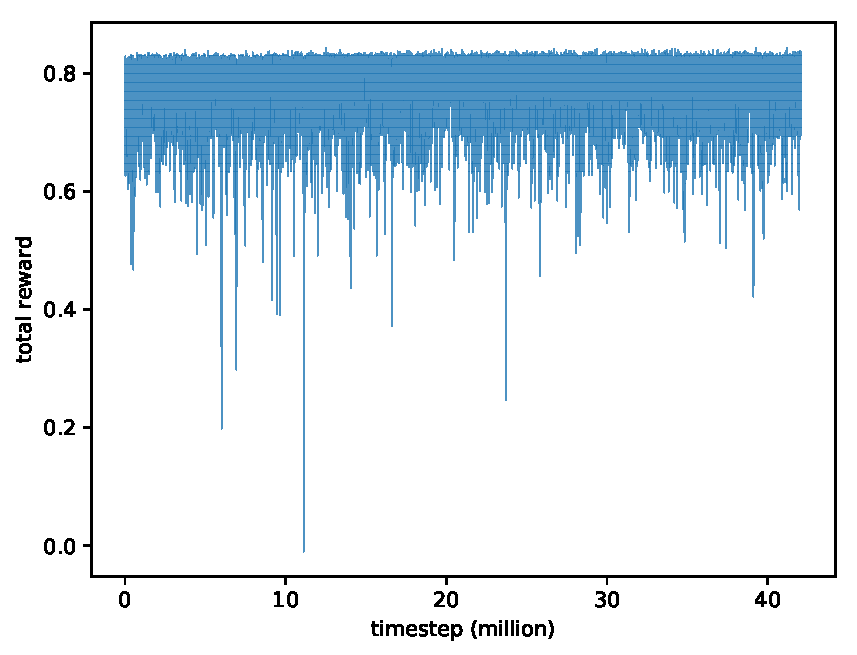
\includegraphics[width=\linewidth]{rec_180711_reachcont_switcher}
	\caption{Switcher policy training performance of the task reachcont, the horizontal axis is the number of million time-steps and the vertical axis is the total episode reward averaged over the last 32 episodes}
	\label{fig:rec_reachcont_switcher}
\end{figure}
\begin{figure}[!htbp]
	\centering
	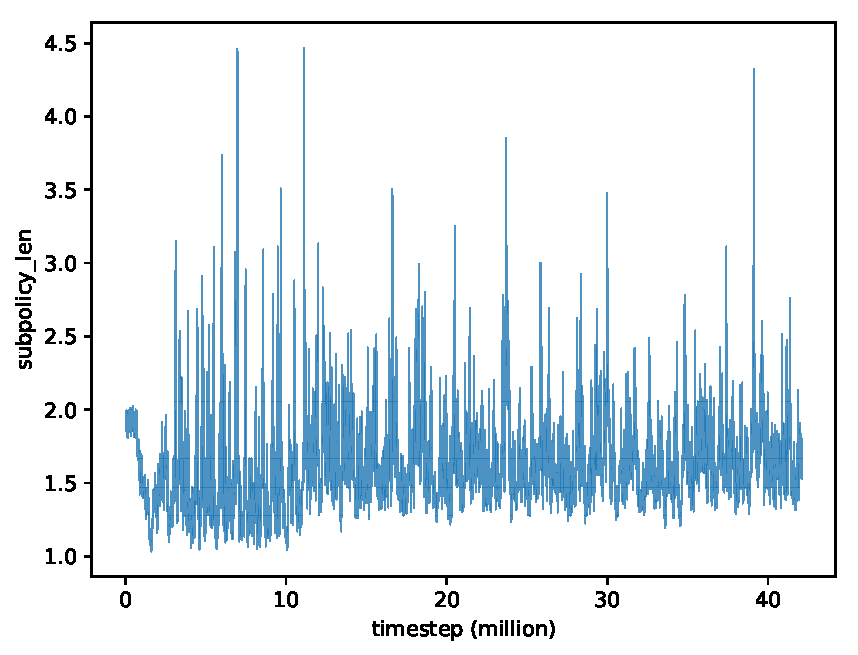
\includegraphics[width=\linewidth]{rec_180711_reachcont_switcher_subt}
	\caption{Average execution length of the actions of decision policies of the task reachcont, the horizontal axis is the number of million time-steps and the vertical axis is the decision policy's average execution length of the last batch.}
	\label{fig:rec_reachcont_switcher_subt}
\end{figure}

The performance of the reachcontreg switcher policy is shown in Figure~\ref{rec_switcher_reachcontreg} and the average execution length of actuator policies is shown in Figure~\ref{rec_switcher_subt_reachcontreg}. A video recording of the agent can be viewed at the website:  [\url{https://youtu.be/Y0uHEpJ7Cck}]. The best performance, which as 95, surpasses the final performance of 70 in phase 1. The average execution length is 1.0 when the performance reaches the highest level. This means that temporal abstraction is also infeasible for this task. The training also follows a pattern that the performance degrades in the later phase of training when the average execution length begins to increase.
\begin{figure}[!htbp]
	\centering
	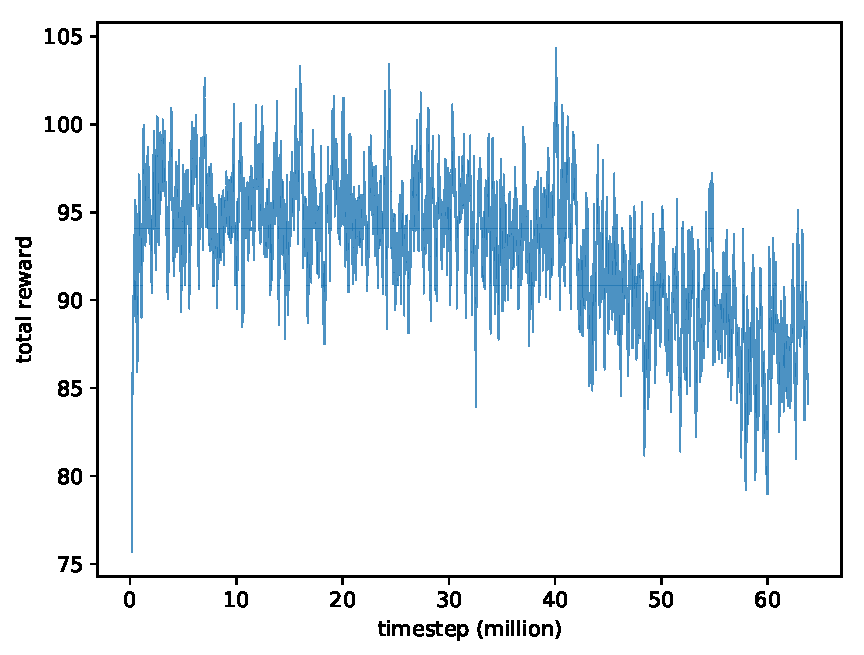
\includegraphics[width=\linewidth]{rec_180719_switcher_reachcontreg}
	\caption{Switcher policy training performance of the task reachcontreg, the horizontal axis is the number of million time-steps and the vertical axis is the total episode reward averaged over the last 200 episodes}
	\label{rec_switcher_reachcontreg}
\end{figure}

\begin{figure}[!htbp]
	\centering
	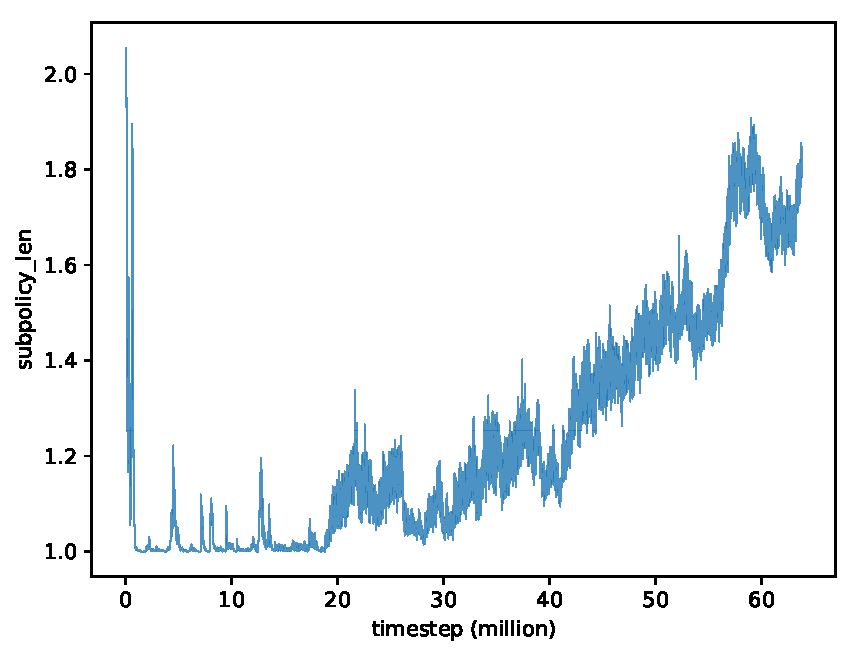
\includegraphics[width=\linewidth]{rec_180719_switcher_subt_reachcontreg}
	\caption{Average execution length of the actions of decision policies of the task reachcontreg, the horizontal axis is the number of million time-steps and the vertical axis is the decision policy's average execution length of the last batch.}
	\label{rec_switcher_subt_reachcontreg}
\end{figure}

One reason that the performance degrades in the late phase of switcher policy training could be due to the regularization term that penalizes the termination of the current actuator policy. The term could have a stronger impact at the late phase of training, where the scale of the advantage term in the reinforcement learning loss decreases.

The above experiment results show that it is feasible to train a switcher policy that controls the scheduling intervals of the decision policy in an end-to-end manner. However, the proposed regularization term does not appear to be an optimal choice. 